\section{Diagrama de conexiones}

Este diagrama representa la interconexion entre los diferentes modulos digitales y analogicos que forman
parte de una experiencia planificada.

\begin{figure}[!htb].
    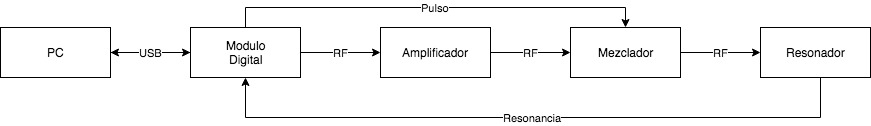
\includegraphics[width=\linewidth]{../figures/d4.jpg}
    \caption{Diagrama de conexiones}
    \label{fig:d4}
\end{figure}
  
%Figure \ref{fig:boat1} shows a boat.

\subsection{Mixer}

Los pulsos de salida y la señal de radiofrecuencia son las entradas del mezclador
donde se convierten en una sola cuando el pulso TTL esta activo en 5 voltios.
Esto permite crear pulsos de estimulacion y relajacion con presicion.

\subsection{Amplificador}


\subsection{Resonador}



\newpage
